% ######################################################################################################################
%         Clustering
% ######################################################################################################################

\chapter{Clustering}
\label{ch:Clustering}

\paperbox{
    This chapter is based on the peer-reviewed publication:
}{\paperpppp}{
    \textbf{Contributions:} Lucas Czech... Alexandros Stamatakis...
}

\todo{distance measures, nhd, simulations, mantel test}

% ######################################################################################################################
%         Motivation
% ######################################################################################################################

\section{Motivation}
\label{ch:Clustering:sec:Motivation}

Given a set of metagenomic samples, one key question is how much they differ from each other.
% Using the phylogenetic placement of the sequences in the samples,
% this question can be answered by...
% For this, we need to devise distance measures between samples.
% For phylogenetic placements, we need to quantify how much the distribution of masses
% differs across the \ac{RT} between two or more samples.
A common distance metric between microbial communities
is the (weighted) UniFrac distance \cite{Lozupone2005,Lozupone2007a}.
It uses the fraction of unique and shared branch lengths between phylogenetic trees to determine their difference.
UniFrac has been generalized and adapted to phylogenetic placements
in form of the phylogenetic Kantorovich-Rubinstein (KR) distance \cite{Matsen2011a,Evans2012}.
In other contexts, the KR distance is also called Wasserstein distance, Mallows distance, or Earth Mover's distance
\cite{Mallows1972,Rachev1985,Levina2001,Villani2008}.
The KR distance between two metagenomic samples is a metric that describes
by at least how much the normalized mass distribution of one sample has to be moved across the \ac{RT}
to obtain the distribution of the other sample.
%In other words, it is the minimum work needed to solve the transportation problem between the two distributions.
% The distance increases with the amount and the displacement of moved mass.
The distance is symmetrical, and becomes larger the more mass needs to be moved,
and the larger the respective displacement (moving distance) is.
% It is thus a natural way of comparing mass distributions.
As the two samples being compared need to have equal masses,
the KR distance operates on normalized samples;
that is, it compares relative abundances.

Given such a distance measure between samples,
% e.g. Earth Mover's Distance or Node Histogram Distance as described above,
a fundamental task consists in clustering samples that are similar to each other.
Standard linkage-based clustering methods like \mbox{UPGMA} % mbox avoids hyphenation
\cite{Michener1957,Sokal1958,Legendre1998} are solely based on the distances between samples,
that is, they calculate the distances of clusters as a function of pairwise sample distances.
Squash Clustering \cite{Matsen2011a,Srinivasan2012} is a method that
also takes into account the intrinsic structure of phylogenetic placement data.
It uses the KR distance to perform agglomerative hierarchical clustering of samples.
Instead of using pairwise sample distances, however,
it merges (\emph{squashes}) clusters of samples by calculating their average per-edge placement mass.
Thus, in each step, it operates on the same type of data, that is, on mass distributions on the \ac{RT}.
This results in a hierarchical clustering tree that has meaningful, and hence interpretable, branch lengths.

Remark:
Squash clustering uses the KR distance, which is based on mass distributions on the edges of the \ac{RT}.
It thus ``suffers'' from the same shortcomings that Edge PCA is solving by using mass imbalance instead.
For instance, Figure 7 of \cite{Matsen2011a} shows the result of a normal principal component analysis
on a dataset of Bacterial Vaginosis, a disease of the vagina.
On the left hand side of the figure, the blue data points, representing healthy women, cluster close together,
while the red data points, which belong to sick patients, spread over the rest of the graph.
The result of Squash Clustering on this dataset is presented in Figure 1 of \cite{Srinivasan2012}.
The bottom half of the clustering tree, containing mainly healthy samples, has short branches,
while the top half, with mostly samples from sick patients, has many long branches.
Thus, Squash Clustering and normal PCA represent almost equivalent information in this case.

% ######################################################################################################################
%         Phylogenetic k-means
% ######################################################################################################################

% PDF bookmarks do not accept the $k$ math mode, so make it use the letter instead.
\section{Phylogenetic \texorpdfstring{$k$-means}{k-means}}
\label{ch:Clustering:sec:PhylogeneticKmeans}

The number of tips in the resulting clustering tree obtained through Squash Clustering
is equal to the number $n$ of samples that are being clustered.
Thus, for datasets with more than a few hundred samples,
the clustering result becomes hard to inspect and interpret visually.
We propose a variant of $k$-means clustering \cite{Macqueen1967} to address this problem,
which we call \emph{Phylogenetic $k$-means}.
It uses a similar approach as Squash Clustering, but yields a predefined number of $k$ clusters.
It is hence able to work with arbitrarily large datasets.
Note that we are clustering samples here, instead of sequences \cite{Kelley2010}.
We discuss choosing a reasonable value for $k$ later.

The underlying idea is to assign each of the $n$ samples to one of $k$ cluster centroids,
where each centroid represents the average mass distribution of all samples assigned to it.
Note that all samples and centroids are of the same data type,
namely, they are mass distributions on a fixed \ac{RT}.
It is thus possible to calculate distances between samples and centroids,
and to calculate their average mass distributions, as described earlier.
Our implementation follows Lloyd's algorithm \cite{Lloyd1982},
% to iteratively improve the assignments and the centroids,
as shown in \algref{algo:kmeans}.

\vspace*{1em} % \todo{maybe remove later again}
\begin{algorithm}
\caption{Phylogenetic $k$-means}\label{algo:kmeans}
\begin{algorithmic}[1]
    \State $ \text{initialize } \textit{k Centroids} $
    \While{ $\text{not converged}$ }
        \State $ \text{assign each } \textit{Sample} \text{ to nearest } \textit{Centroid} $
        \State $ \text{update } \textit{Centroids} \text{ as mass averages of their } \textit{Samples} $
    \EndWhile
    \State \textbf{return} \text{Assignments and} $\textit{Centroids}$
\end{algorithmic}
\end{algorithm}

By default, we use the $k$-means++ initialization algorithm \cite{Arthur2007} to obtain a set of $k$ initial centroids.
It works by subsequent random selection of samples to be used as initial centroids,
until $k$ centroids have been selected.
In each step, the probability of selecting a sample is
proportional to its squared distance to the nearest already selected sample.
An alternative initialization is to select samples as initial clusters entirely at random.
This is however more likely to yield sub-optimal clusterings \cite{Kanungo2003}.

Then, each sample is assigned to its nearest centroid, using the KR distance. %for example the KR or NH distance.
Lastly, the centroids are updated to represent
the average mass distribution of all samples that are currently assigned to them.
This iterative process alternates between improving the assignments and the centroids.
Thus, the main difference to normal $k$-means is the use of phylogenetic information:
Instead of euclidean distances on vectors, we use the KR distance,
and instead of averaging vectors to obtain centroids, we use the average mass distribution.

The process is repeated until it converges,
that is, the cluster assignments do not change any more,
or until a maximum number of iterations have been executed.
% The second stopping criterion makes sure that the algorithm terminates even with non-convergent datasets.
The second stopping criterion is added to avoid the super-polynomial worst case running time of $k$-means,
which however almost never occurs in practice \cite{Bottou1995,Arthur2006}.

The result of the algorithm is an assignment of each sample to one of the $k$ clusters.
As the algorithm relies on the KR distance, it clusters samples with similar relative abundances.
The cluster centroids can be visualized as trees with a mass distribution,
analogous to how Squash Clustering visualizes inner nodes of the clustering tree.
That is, each centroid can be represented as the average mass distribution of the samples that were assigned to it.
This allows to inspect the centroids and thus to interpret how the samples were clustered.
Examples of this are shown in \figref{fig:centroids}.

The key question is how to select an appropriate $k$
that reflects the number of ``natural'' clusters in the data.
There exist various suggestions in the literature
\cite{Thorndike1953,Rousseeuw1987,Bischof1999,Pelleg2000,Tibshirani2001,Hamerly2004};
% See also: https://stackoverflow.com/a/1793572/4184258 and
% http://www.sthda.com/english/articles/29-cluster-validation-essentials/96-determining-the-optimal-number-of-clusters-3-must-know-methods/
we assessed the Elbow method \cite{Thorndike1953} as explained in \figref{fig:elbows},
which is a straight forward method that yielded reasonable results for our test datasets.
Additionally, for a quantitative evaluation of the clusterings,
we used the $k$ that arose from the number of distinct labels based on the available meta-data for the data.
% that is, the number of distinct categories our data is known to belong to.
For example, the \ac{HMP} samples are labeled with \num{18} distinct body sites,
describing where each sample was taken from, c.f.~\figref{fig:hmp_kmeans_all_18}.

% ======================================================================================================================
%     Algorithmic Improvements
% ======================================================================================================================

\subsection{Algorithmic Improvements}
\label{ch:Clustering:sec:PhylogeneticKmeans:sub:AlgorithmicImprovements}

In each assignment step of the algorithm, distances from all samples to all centroids are calculated,
which has a time complexity of $\mathcal{O}(n \cdot k)$.
In order to accelerate this step, we can apply branch binning
as introduced in \secref{ch:Foundations:sec:PhylogeneticPlacement:sub:PlacementProcessing:par:EdgeMasses}.
% It is both possible to bin all samples, or just the centroid masses,
% but not the samples, as an intermediate approximation.
For the \ac{BV} dataset, we found that even using just \num{2} bins per edge does not alter the cluster assignments.
Branch binning reduces the number of mass points that have to be accessed in memory during KR distance calculations;
however, the costs for tree traversals remain.
Thus, we observed a maximal speedup of 75\% when using one bin per branch,
see \tabref{tab:hmp_binning_error} for details.
% even binning to \num{1} bin,
% that is, combining all placement masses on a branch into one point,
% changes the cluster assignment of only \num{2} of {220} samples
% -- both of which were near the border between two clusters.
% The main bottleneck in the computation however seems to be
% the random memory access to the edges and per-edge masses induced by the tree traversals
% so that binning does not yield substantial speedups.
% In our tests, summarizing all masses in one bin per branch resulted in a speedup of around 75\%,

Furthermore, during the execution of the algorithm, empty clusters can occur,
for example, if $k$ is greater than the number of natural clusters in the data.
Although this problem did not occur in our tests, we implemented the following solution:
First, find the cluster with the highest variance.
Then, choose the sample of that cluster that is furthest from its centroid,
and assign it to the empty cluster instead.
This process is repeated if multiple empty clusters occur at once.

% ######################################################################################################################
%         Imbalance k-means
% ######################################################################################################################

% PDF bookmarks do not accept the $k$ math mode, so make it use the letter instead.
\section{Imbalance \texorpdfstring{$k$-means}{k-means}}
\label{ch:Clustering:sec:ImbalanceKmeans}

We further propose \emph{Imbalance $k$-means},
which is a variant of $k$-means that makes use of the edge imbalance transformation,
and thus also takes the clades of the tree into account.
In order to quantify the difference in imbalances between two samples,
we use the euclidean distance between their imbalance vectors (that is, rows of the imbalance matrix).
This is a suitable distance measure,
as the imbalances implicitly capture the tree topology as well as the placement mass distributions.
As a consequence, the expensive tree traversals required for Phylogenetic $k$-means are not necessary here.
The algorithm takes the edge imbalance matrix of normalized samples as input,
as shown in \figref{fig:imbalance:sub:Matrices},
and performs a standard euclidean $k$-means clustering following Lloyd's algorithm.
% As there is no apparent phylogenetically informative distance measure between imbalance vectors,
% we use euclidean distance instead.
% This also allows to calculated centroids as simple vector averages.

This variant of $k$-means tends to find clusters that are consistent with the results of Edge PCA,
as both use the same input data as well as the same distance measure.
Furthermore, as the method does not need to calculate KR distances,
and thus does not involve tree traversals,
it is several orders of magnitude faster than the Phylogenetic $k$-means.
For example, on the \ac{HMP} dataset, it runs in mere seconds, instead of several hours needed for Phylogenetic $k$-means;
see Section \nameref{ch:Clustering:sec:Results:sub:Performance} for details.
% \todo{die nameref links, die von diesem dummen template erwartet werden, sind nicht eindeutig.
% das ist nicht gut, muss mir da mal was ausdenken, oder noch mal im submission guide nachschauen...}

% ######################################################################################################################
%         Results
% ######################################################################################################################

\section{Results}
\label{ch:Clustering:sec:Results}

We now evaluate our Phylogenetic $k$-means clustering (which uses edge masses and KR distances) and
Imbalance $k$-means clustering (which uses edge imbalances and euclidean distances) methods in terms of their clustering accuracy.
We used the \ac{BV} as an example of a small dataset to which methods such as Squash Clustering \cite{Matsen2011a} are still applicable,
and the \ac{HMP} dataset to showcase that our methods scale to datasets that are too large for existing methods.

% ----------------------------------------------------------------------------------------------------------------------
%     BV Dataset
% ----------------------------------------------------------------------------------------------------------------------

\subsection{BV Dataset}
\label{ch:Clustering:sec:Results:sub:BVDataset}

We again use the re-analyzed \ac{BV} dataset to test whether our methods work as expected,
by comparing them to the existing analysis of the data in \cite{Srinivasan2012} and \cite{Matsen2011a}.
To this end, we ran both Phylogenetic $k$-means and Imbalance $k$-means on the \ac{BV} dataset.
We chose $k:=3$, inspired by the findings of \cite{Srinivasan2012}.
They distinguish between subjects affected by Bacterial Vaginosis and healthy subjects,
and further separate the healthy ones into two categories depending on the dominating clade in the vaginal microbiome,
which is either \taxonname{Lactobacillus iners} or \taxonname{Lactobacillus crispatus}.
Any choice of $k > 3$ would simply result in smaller, more fine-grained clusters,
but not change the general findings of these experiments.
An evaluation of the number of clusters using the Elbow method is shown in \figref{fig:elbows}.
We furthermore conducted Squash Clustering and Edge PCA on the dataset,
thereby reproducing previous results, in order to allow for a direct comparison between the methods,
see \figref{fig:cluster_kmeans}.
The figure shows the results of Squash Clustering, Edge PCA, and two alternative dimensionality reduction methods,
colorized by the cluster assignments \emph{PKM} of Phylogenetic $k$-means (in red, green, and blue)
and \emph{IKM} of the Imbalance $k$-means (in purple, orange, and gray), respectively.
We use two different color sets for the two methods, in order to make them distinguishable at first glance.
Note that the mapping of colors to clusters is arbitrary and depends on the random initialization of the algorithm.

% That figure is bonkers. Everything condensed in half a page. I like it!
\begin{figure}[!ht]
    \centering
    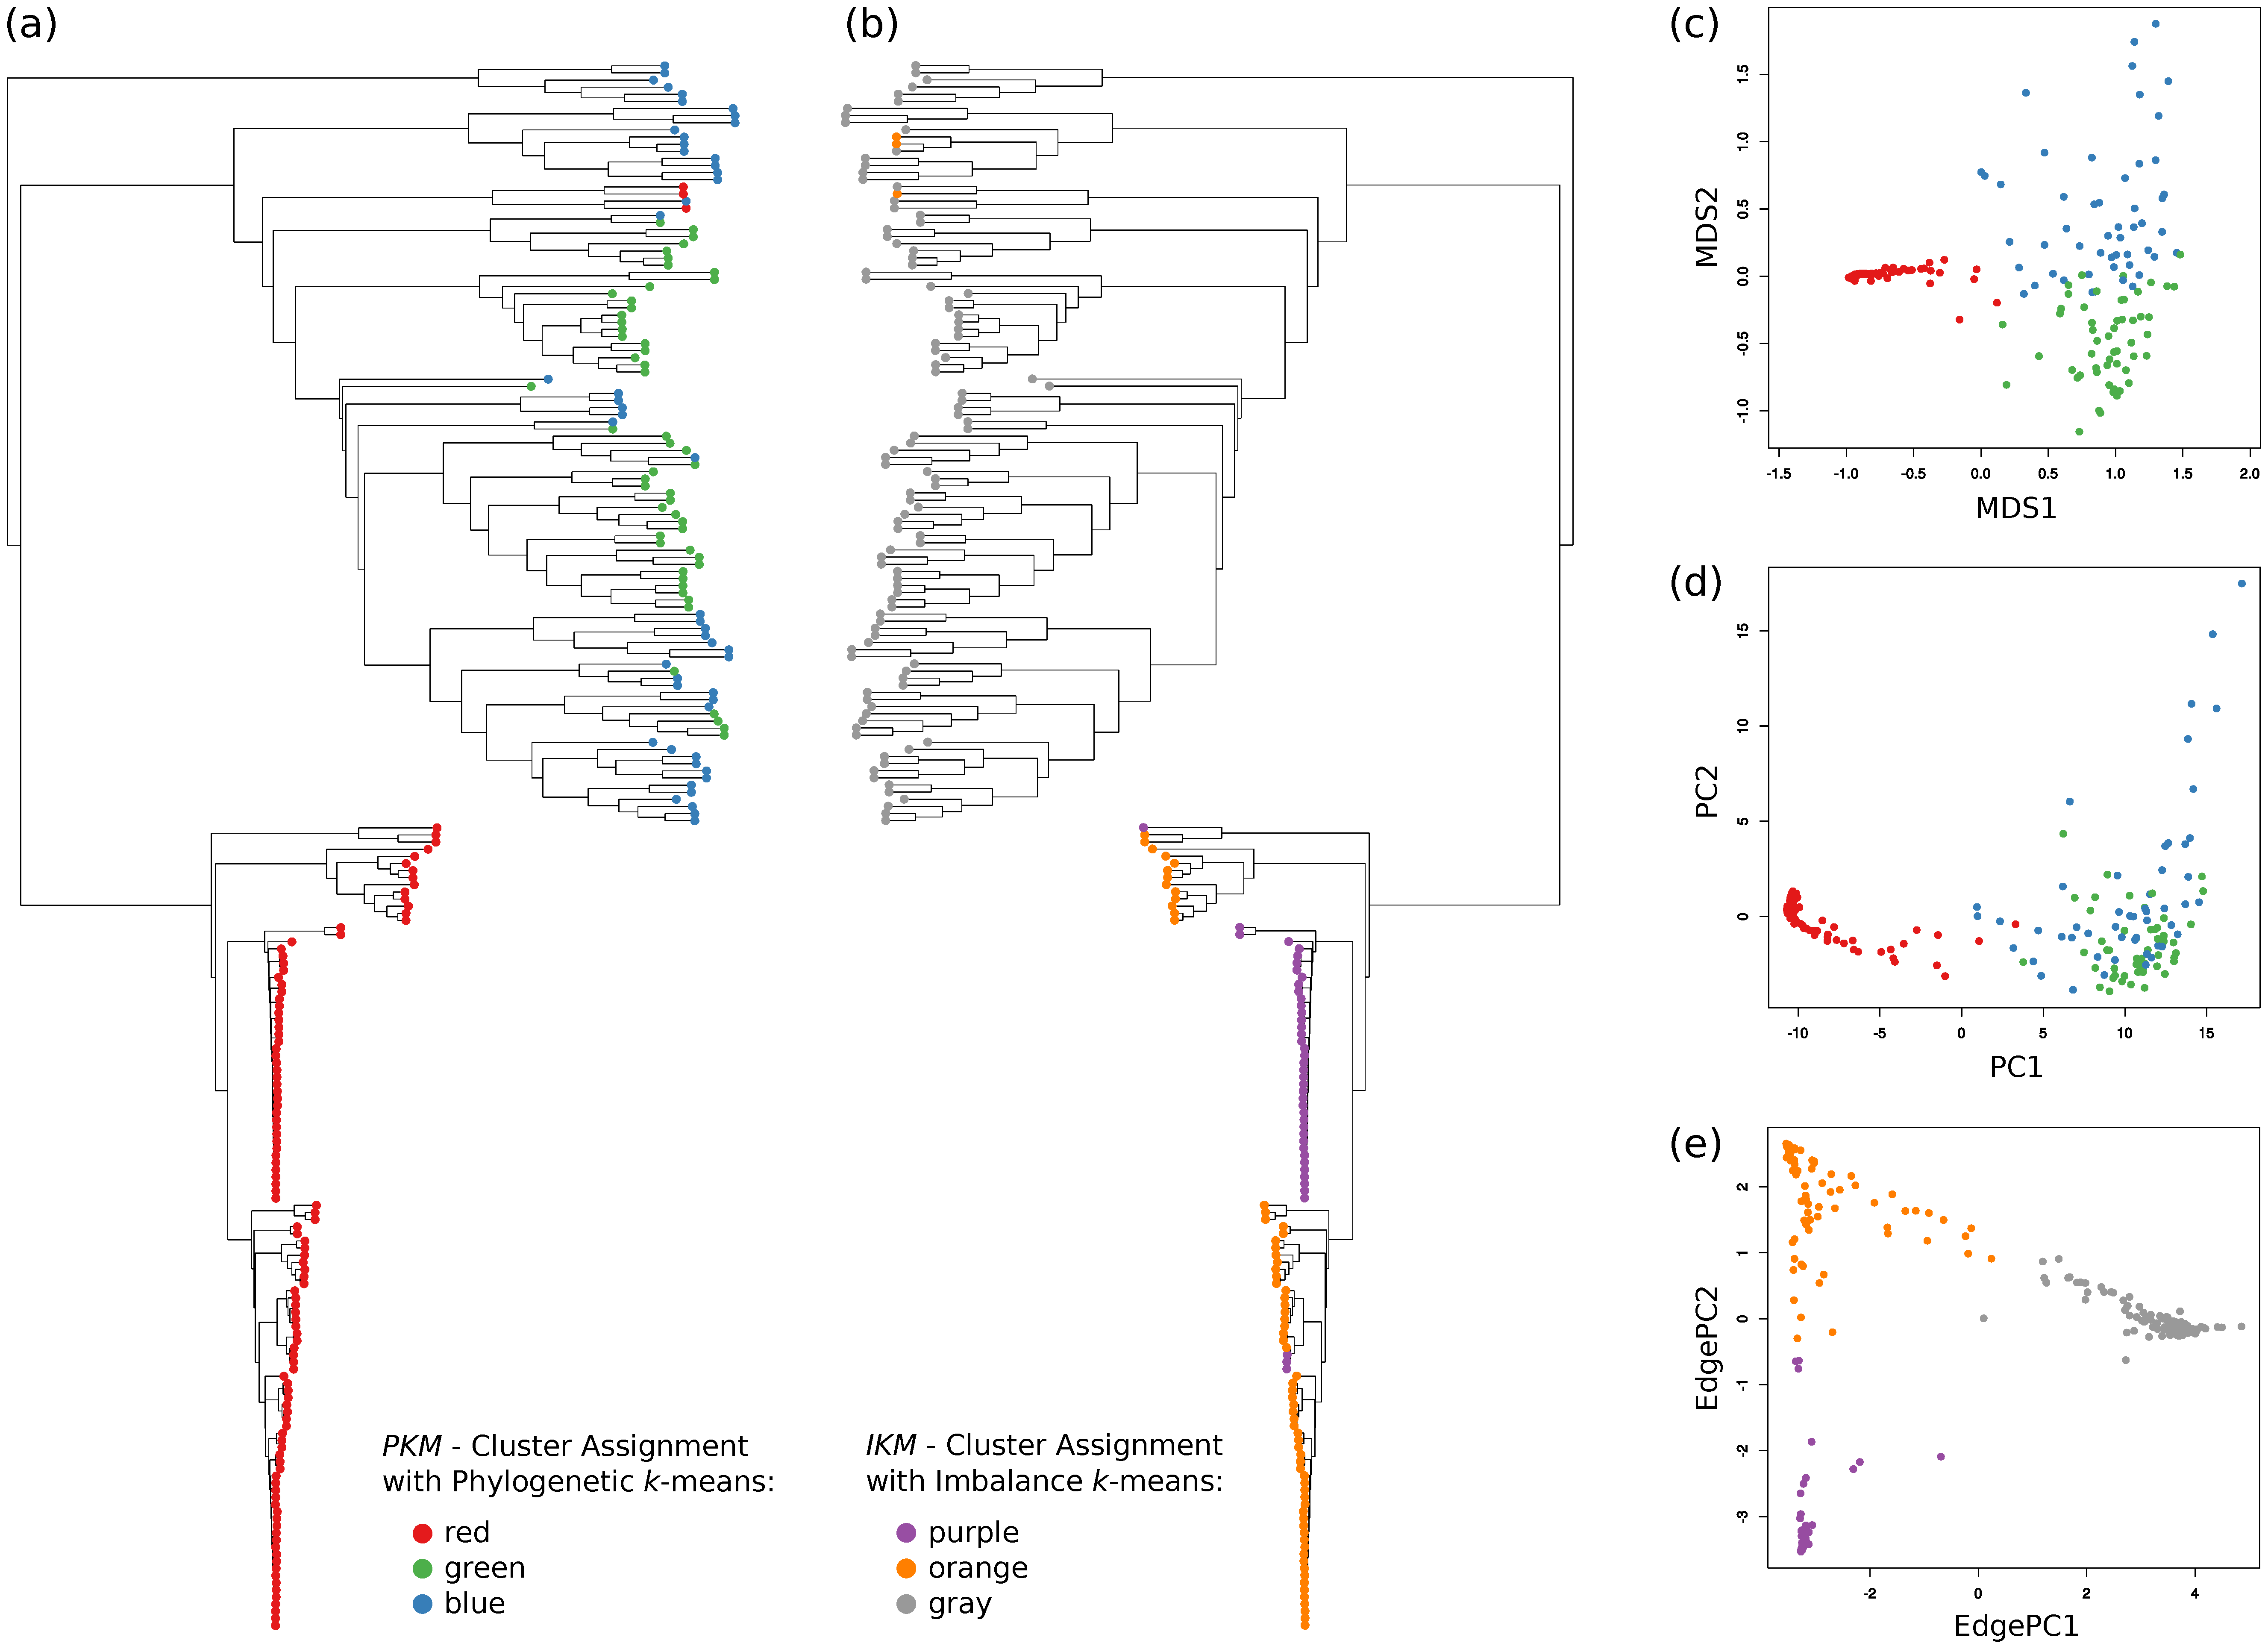
\includegraphics[width=\linewidth]{pppp/cluster_kmeans.pdf}
    \begin{subfigure}{0pt}
        \phantomcaption
        \label{fig:cluster_kmeans:sub:mass_tree}
    \end{subfigure}
    \begin{subfigure}{0pt}
        \phantomcaption
        \label{fig:cluster_kmeans:sub:imbalance_tree}
    \end{subfigure}
    \begin{subfigure}{0pt}
        \phantomcaption
        \label{fig:cluster_kmeans:sub:mds}
    \end{subfigure}
    \begin{subfigure}{0pt}
        \phantomcaption
        \label{fig:cluster_kmeans:sub:pca}
    \end{subfigure}
    \begin{subfigure}{0pt}
        \phantomcaption
        \label{fig:cluster_kmeans:sub:edgepca}
    \end{subfigure}
    \caption[Comparison of $k$-means clustering to Squash Clustering and Edge PCA]{
        \textbf{Comparison of $k$-means clustering to Squash Clustering and Edge PCA.}
        We applied our variants of the $k$-means clustering method
        to the \ac{BV} dataset in order to compare them to existing methods.
        See \cite{Srinivasan2012} for details of the dataset and its interpretation.
        We chose $k:=3$, as this best fits the features of the dataset.
        For each sample, we obtained two cluster assignments:
        First, by using Phylogenetic $k$-means, %that is, by using edge masses as input to $k$-means,
        we obtained the cluster assignment \emph{PKM}.
        Second, by using Imbalance $k$-means, we obtained assignment \emph{IKM}.
        In each subfigure, the \num{220} samples are represented by colored circles:
        red, green, and blue show the cluster assignments \emph{PKM},
        while purple, orange, and gray show the cluster assignments \emph{IKM}.
        % Sub (A)
        \subref{fig:cluster_kmeans:sub:mass_tree}
        Hierarchical cluster tree of the samples, using Squash Clustering.
        The tree is a recalculation of Figure~1(A) of \cite{Srinivasan2012}.
        Each leaf represents a sample; branch lengths are KR distances.
        We added color coding for the samples, using \emph{PKM}.
        The lower half of red samples are mostly healthy subjects,
        while the green and blue upper half are patients affected by Bacterial Vaginosis.
        % Sub (B)
        \subref{fig:cluster_kmeans:sub:imbalance_tree}
        The same tree, but annotated by \emph{IKM}.
        The tree is flipped horizontally for ease of comparison.
        The healthy subjects are split into two sub-classes,
        discriminated by the dominating species in their vaginal microbiome:
        orange and purple represent samples were \taxonname{Lactobacillus iners} and \taxonname{Lactobacillus crispatus}
        dominate the microbiome, respectively.
        The patients mostly affected by BV are clustered in gray.
        % Sub (C)
        \subref{fig:cluster_kmeans:sub:mds}
        Multidimensional scaling using the pairwise KR distance matrix of the samples,
        and colored by \emph{PKM}.
        % Sub (D)
        \subref{fig:cluster_kmeans:sub:pca}
        Principal component analysis applied to the distance matrix by interpreting it as a data matrix.
        This is a recalculation of Figure~4 of \cite{Matsen2011b},
        but colored by \emph{PKM}.
        % Sub (E)
        \subref{fig:cluster_kmeans:sub:edgepca}
        Edge PCA applied to the samples,
        which is a recalculation of Figure~3 of \cite{Matsen2011b},
        but colored by \emph{IKM}.
    }
    \label{fig:cluster_kmeans}
\end{figure}

As can be seen in \figref{fig:cluster_kmeans:sub:mass_tree}, Squash Clustering as well as
Phylogenetic $k$-means can distinguish healthy subjects from those affected by Bacterial Vaginosis.
Healthy subjects constitute the lower part of the cluster tree.
They have shorter branches between each other, indicating the smaller KR distance between them,
which is a result of the dominance of \taxonname{Lactobacillus} in healthy subjects.
The same clusters are found by Phylogenetic $k$-means:
As it uses the KR distance, it assigns all healthy subjects with short cluster tree branches to one cluster (shown in red).
The green and blue clusters are mostly the subjects affected by the disease.

The distinguishing features between the green and the blue cluster are not apparent in the Squash cluster tree.
This can however be seen in \figref{fig:cluster_kmeans:sub:mds},
which shows a \acf{MDS} plot of the pairwise KR distances between the samples.
\ac{MDS} \cite{Mardia1978,Krzanowski1994,Everitt2010} is a dimensionality reduction method that
can be used for visualizing levels of similarity between data points.
Given a pairwise distance matrix, it finds an embedding into lower dimensions (in this case, \num{2} dimensions)
that preserves higher dimensional distances as well as possible.
Here, the red cluster forms a dense region, which is in agreement with its short branch lengths
in the cluster tree.
At the same time, the green and blue cluster are separated in the \ac{MDS} plot,
but form a coherent region of low density,
indicating that $k:=3$ might be too large with Phylogenetic $k$-means on this dataset.
That is, the actual clustering just distinguishes healthy from sick patients (\figref{fig:elbows}).
% which, albeit not well separated from each other, indicate groups of samples with lower KR distance between each other.
% Although this separation is smooth, it shows how Phylogenetic $k$-means
% finds clusters based on KR distance between samples, and thus yields results comparable to \ac{MDS}.

A similar visualization of the pairwise KR distances is shown in \figref{fig:cluster_kmeans:sub:pca}.
It is a recalculation of Figure~4 in the preprint \cite{Matsen2011b},
which did not appear in the final published version \cite{Matsen2011a}.
% Alternatively:
It is a recalculation of Figure~4 of \cite{Matsen2011b}.
but can also be found at \cite{MatsenEdgePCA}.
The figure shows a standard \acf{PCA} \cite{Krzanowski1994,Everitt2010} applied to the distance matrix
by interpreting it as a data matrix, and was previously used to motivate Edge PCA.
However, although it is mathematically sound,
the direct application of \ac{PCA} to a distance matrix lacks a simple interpretation.
Again, the red cluster is clearly separated from the rest,
but this time, the distinction between the green and the blue cluster is not as apparent.

In \figref{fig:cluster_kmeans:sub:imbalance_tree}, we compare Squash Clustering to Imbalance $k$-means.
Here, the distinction between the two \taxonname{Lactobacillus} clades
can be seen by the purple and orange cluster assignments.
The cluster tree also separates those clusters into clades.
The separate small group of orange samples above the purple clade is an artifact of the tree ladderization.
The diseased subjects are all assigned to the gray cluster, represented by the upper half of the cluster tree.
It is apparent that both methods separate the same samples from each other.

Lastly, \figref{fig:cluster_kmeans:sub:edgepca} compares Imbalance $k$-means to Edge PCA.
The plot is a recalculation of Figure~3 of \cite{Matsen2011b}, which also appeared in Figure~6 in \cite{Matsen2011a}
and Figure~3 in \cite{Srinivasan2012},
but colored using our cluster assignments.
Because both methods work on edge imbalances, they group the data in the same way,
that is, they clearly separate the two healthy groups and the diseased one from each other.
Edge PCA forms a plot with three corners, which are colored by the three Imbalance $k$-means cluster assignments.

In \figref{fig:kmeans_all}, we report more details of the comparison of our $k$-means variants
to the dimensionality reduction methods used here.
Furthermore, examples visualizations of the cluster centroids are shown in \figref{fig:centroids},
which further supports that our methods yield results that are in agreement with existing methods.
% In summary, our novel $k$-means variants find clusters that are in agreement with existing methods.
% \todo{cluster centroid diversity ist interessant. plus tax assignment counts a la pierre pro centroid.}

% ----------------------------------------------------------------------------------------------------------------------
%     HMP Dataset
% ----------------------------------------------------------------------------------------------------------------------

\subsection{HMP Dataset}
\label{ch:Clustering:sec:Results:sub:HMPDataset}

The \ac{HMP} dataset is used here as an example to show that our method scales to large datasets.
To this end, we used the unconstrained \taxonname{Bacteria} \ac{RT} with \num{1 914} taxa
as provided by our Automatic Reference Tree method \cite{Czech2018}.
The tree represents a broad taxonomic range of \taxonname{Bacteria},
that is, the sequences were not explicitly selected for the \ac{HMP} dataset,
in order to test the robustness of our clustering methods.
We then placed the \num{9 192} samples of the \ac{HMP} dataset with a total of \num{118 701 818} sequences
on that tree, and calculated Phylogenetic and Imbalance $k$-means on the samples.
The freely available meta-data for the \ac{HMP} dataset labels each sample by the body site were it was
taken from.
As there are \num{18} different body site labels, we used $k:=18$.
The result is shown in \figref{fig:hmp_kmeans_all_18}.
Furthermore, in \figref{fig:hmp_kmeans_all_8},
we show a clustering of this dataset into $k:=8$ broader body site regions
to exemplify the effects of using different values of $k$.
This is further explored by using the Elbow method as shown in \figref{fig:elbows}.
% that is, using the constrained Bacterial tree as well as Imbalance $k$-means.

\begin{figure}[hpbt]
    \centering
    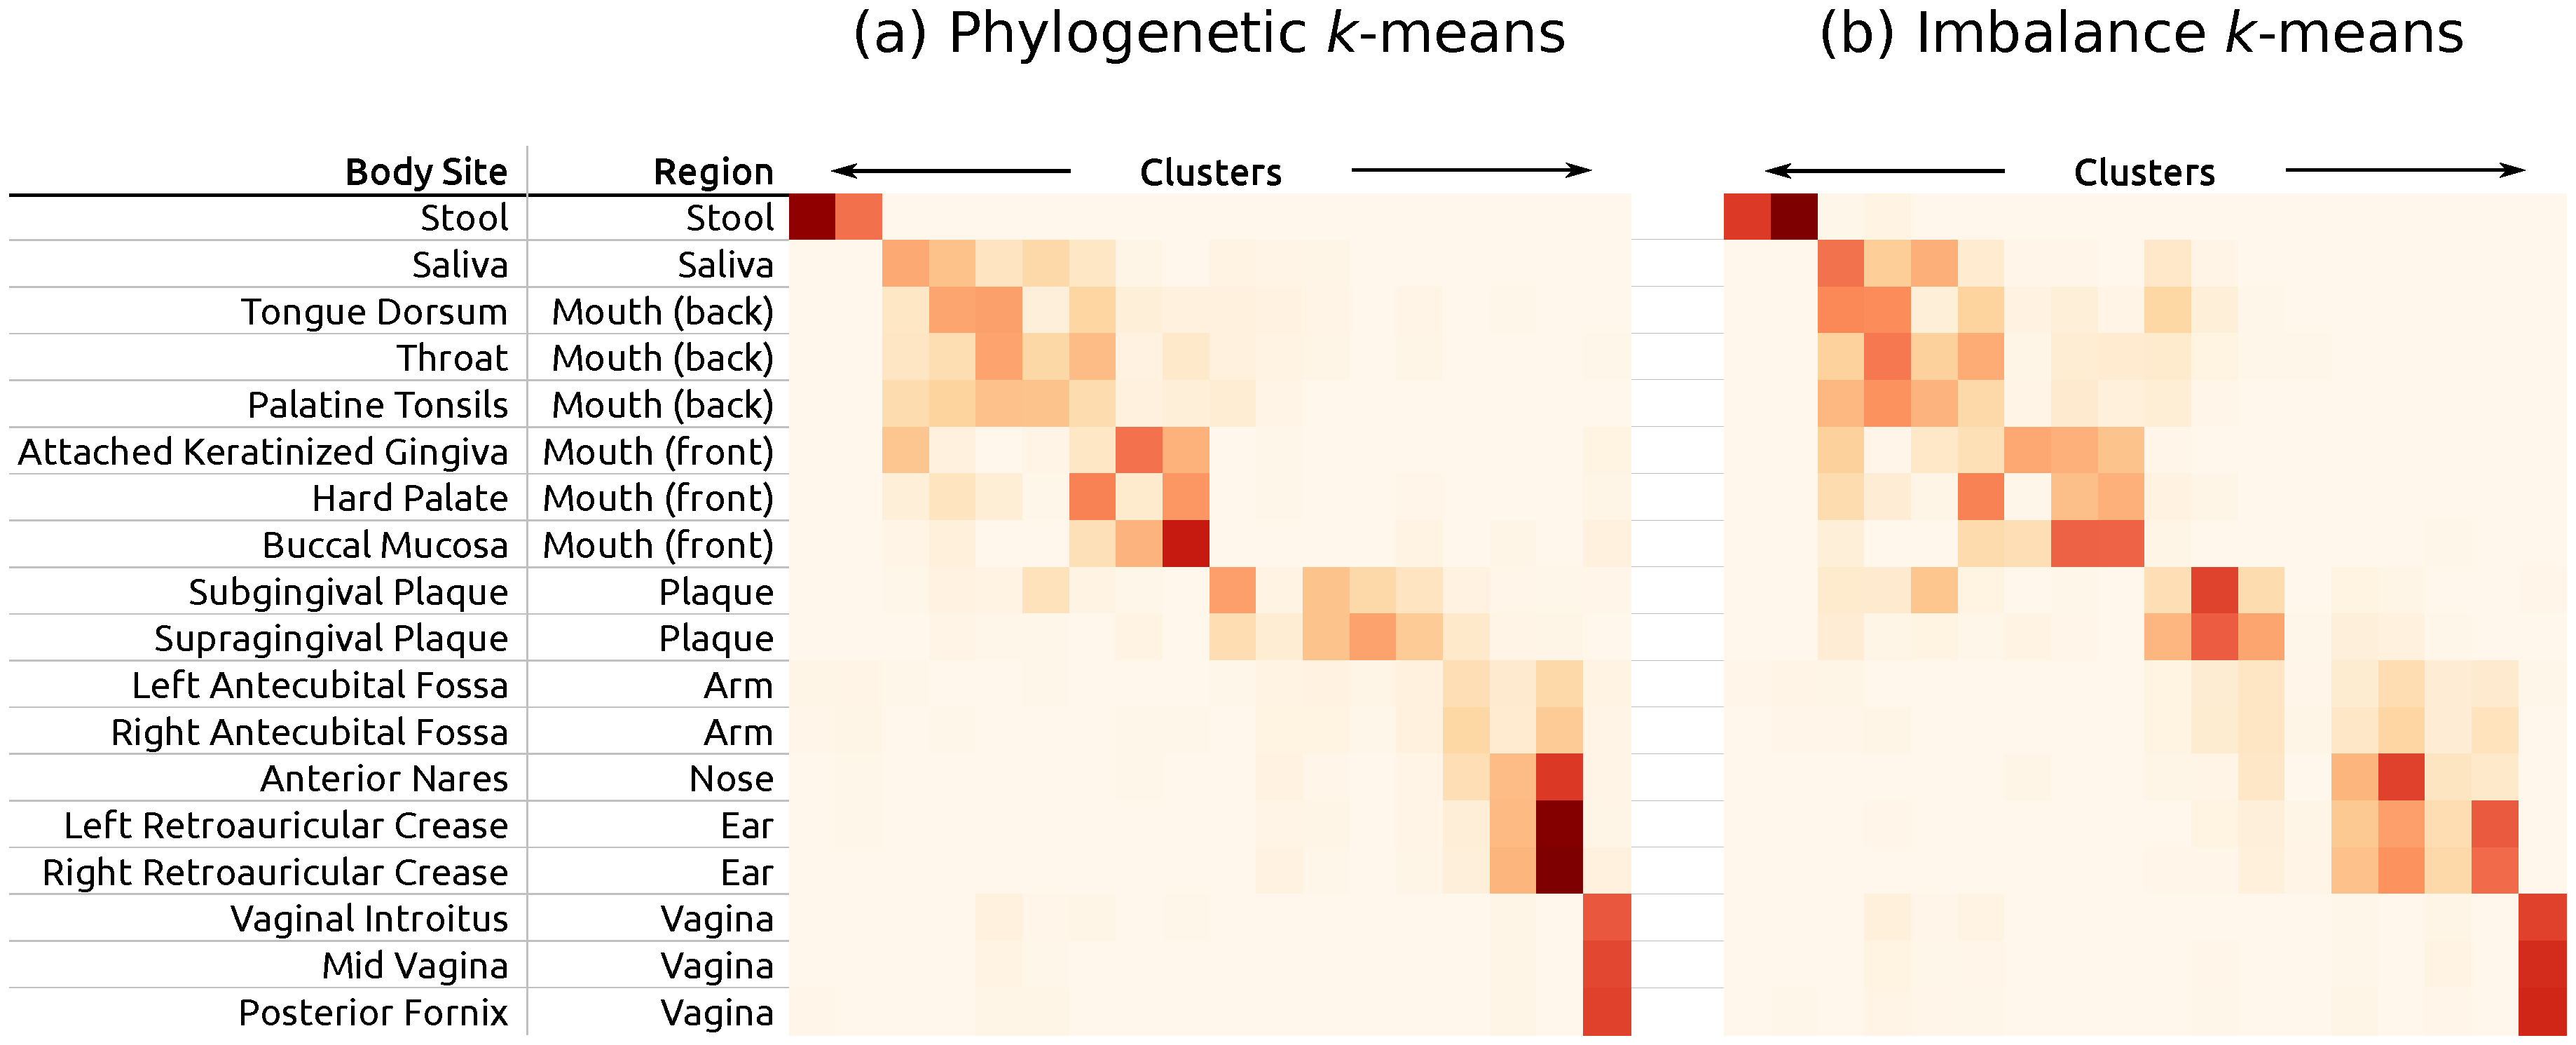
\includegraphics[width=\linewidth]{pppp/hmp_kmeans_all_18.pdf}
    \begin{subfigure}{0pt}
        \phantomcaption
        \label{fig:hmp_kmeans_all_18:sub:em_unconstr}
    \end{subfigure}
    \begin{subfigure}{0pt}
        \phantomcaption
        \label{fig:hmp_kmeans_all_18:sub:ei_unconstr}
    \end{subfigure}
    \caption[$k$-means cluster assignments of the \ac{HMP} dataset with $k:=18$]{
        \textbf{$k$-means cluster assignments of the \ac{HMP} dataset with $k:=18$.}
        Here, we show the cluster assignments as yielded by
        Phylogenetic $k$-means \subref{fig:hmp_kmeans_all_18:sub:em_unconstr} and
        Imbalance $k$-means \subref{fig:hmp_kmeans_all_18:sub:ei_unconstr} of the \ac{HMP} dataset.
        We used $k:=18$, which is the number of body site labels in the dataset,
        in order to compare the clusterings to this ``ground truth''.
        Each row represents a body site; each column one of the 18 clusters found by the algorithm.
        The color values indicate how many samples of a body site were assigned to each cluster.
        Similar body sites are clearly grouped together in coherent blocks, indicated by darker colors.
        For example, the stool samples were split into two clusters (topmost row),
        while the three vaginal sites were all put into one cluster (rightmost column).
        However, the algorithm cannot always distinguish between nearby sites,
        as can be seen from the fuzziness of the clusters of oral samples.
        This might be caused by our broad reference tree,
        and could potentially be resolved by using a tree more specialized for the data/region (not tested).
        Lastly, the figure also lists how the body site labels were aggregated into regions
        as used in \figref{fig:hmp_kmeans_all_8}.
        \\
        Although the plots of the two $k$-means variants generally exhibit similar characteristics,
        there are some differences.
        For example, the samples from the body surface (ear, nose, arm)
        form two relatively dense clusters (columns) in \subref{fig:hmp_kmeans_all_18:sub:em_unconstr},
        whereas those sites are spread across four of five clusters in \subref{fig:hmp_kmeans_all_18:sub:ei_unconstr}.
        On the other hand, the mouth samples are more densely clustered in \subref{fig:hmp_kmeans_all_18:sub:ei_unconstr}.
    }
    \label{fig:hmp_kmeans_all_18}
\end{figure}

% Ideally, each cluster would contain only samples from the same body site.
Ideally, all samples from one body site would be assigned to the same cluster,
hence forming a diagonal on the plot.
However, as there are several nearby body sites, which share a large fraction of their microbiome \cite{Huttenhower2012},
we do not expect a perfect clustering.
Furthermore, we used a broad reference tree that might not be able to resolve details in some clades.
% which was originally meant only for a first classification of sequences (see above).
% Thus, the tree does not particularly suit the dataset well.
Nonetheless, the clustering is reasonable, which indicates a robustness against the exact choice of reference taxa,
and can thus by used for distinguishing among samples.
For example, stool and vaginal samples are clearly clustered.
Furthermore, the sites that are on the surface of the body (ear, nose, and arm)
also mostly form two blocks of cluster columns.
% We also evaluated the clustering using the two General trees of our automatic reference trees (data not shown),
% thus using an even less specific set of taxa.
% This yielded cluster assignments which are almost identical to the shown ones, except for slightly more fuzziness.
% We thus expect that the clustering improves when using an \ac{RT}
% containing taxa specifically chosen for the type of sequences in the dataset.
% % This however remains future work.

% ----------------------------------------------------------------------------------------------------------------------
%     Performance
% ----------------------------------------------------------------------------------------------------------------------

\subsection{Performance}
\label{ch:Clustering:sec:Results:sub:Performance}

The complexity of Phylogenetic $k$-means is in $\mathcal{O}(k \cdot i \cdot n \cdot e)$,
with $k$ clusters, $i$ iterations, and $n$ samples, and $e$ being the number of tree edges,
which corresponds to the number of dimensions in standard euclidean $k$-means.
As the centroids are randomly initialized, the number of iterations can vary;
in our tests, it was mostly below \num{100}.
For the \ac{BV} dataset with \num{220} samples and a reference tree with \num{1 590} edges, using $k:=3$,
our implementation ran \num{9} iterations, needing \SI{35}{\second} and \SI{730}{\mega\byte} of main memory on a single core.
For the \ac{HMP} dataset with \num{9 192} samples and \num{3 824} edges, we used $k:=18$,
which took \num{46} iterations and ran in \SI{2.7}{\hour} on \num{16} cores, using \SI{48}{\giga\byte} memory.

In contrast to this, Imbalance $k$-means does not need to conduct any expensive tree traversals,
and instead operates on compact vectors, using euclidean distances.
It is hence several orders of magnitude faster than Phylogenetic $k$-means.
For example, using again $k:=18$ for the \ac{HMP} dataset,
the algorithm executed \num{75} iterations in \SI{2}{\second}.
It is thus also applicable to extremely large datasets.

Furthermore, as the KR distance is used in Phylogenetic $k$-means as well as other methods such as Squash Clustering,
our implementation is highly optimized and
outperforms the existing implementation in \toolname{guppy} \cite{Matsen2010} by orders of magnitude (see below for details).
The KR distance between two samples has a linear computational complexity in both the number of \acp{QS} and the tree size.
As a test case, we computed the pairwise distance matrix between sets of samples.
Calculating this matrix is quadratic in the number of samples,
and is thus expensive for large datasets.
For example, in order to calculate the matrix for the \ac{BV} dataset with \num{220} samples,
\toolname{guppy} can only use a single core and required \SI{86}{\minute}.
Our KR distance implementation in \toolname{genesis} is faster and also supports multiple cores.
It only needed \SI{90}{\second} on a single core; almost half of this time is used for reading input files.
When using \num{32} cores, the matrix calculation itself only took \SI{8}{\second}.
This allows to process larger datasets:
The distance matrix of the \ac{HMP} dataset with \num{9 192} samples placed on a tree with \num{3 824} branches
for instance took less than \SI{10}{\hour} to calculate using \num{16} cores in \toolname{genesis}.
In contrast, \toolname{guppy} needed \num{43} days for this dataset.
% As the KR distance is also used in Squash Clustering,
% our re-implementation of this method is orders of magnitude faster than the original \toolname{guppy} implementation.
% For even bigger datasets, the mass binning method can be used for speedup.
% The performance and the effects of binning on the distance values are explored
% in Section {link to correct sub section of eval. also, performance is now spread}.
Lastly, branch binning can be used to achieve additional speedups,
as shown in \tabref{tab:hmp_binning_error}.

% ######################################################################################################################
%         Conclusion and Outlook
% ######################################################################################################################

\section{Conclusion and Outlook}
\label{ch:Clustering:sec:ConclusionOutlook}

Furthermore, we presented adapted variants of the $k$-means method,
which exploit the structure of phylogenetic placement data to identify clusters of environmental samples.
The method builds upon ideas such as Squash Clustering and can be applied to substantially larger datasets,
as it uses a pre-defined number of clusters.
% They are thus useful to identify similarities between samples
For future exploration, other forms of cluster analyses could be extended to work on phylogenetic placement data,
for example, soft $k$-means clustering \cite{Dunn1973,Bezdek1981} or density-based methods \cite{Kriegel2011}.
The main challenge when adopting such methods consists in making them phylogeny-aware,
that is, to use mass distributions on trees instead of the typical $\mathbb{R}^n$ vectors.
%as the underlying space in which the data is modeled.

% ######################################################################################################################
%         Supplement
% ######################################################################################################################

% ======================================================================================================================
%     Binnify Speedup and Errors
% ======================================================================================================================

\begin{table}[htb]
\caption[Effect of Branch Binning on the KR Distance of the HMP Dataset]{
\textbf{Effect of Branch Binning on the KR Distance of the HMP Dataset.}
Here we show the effect of per-branch placement binning
on the run-time and on the resulting relative error when calculating the pairwise KR distance matrix between samples,
by example of the Human Microbiome Project (HMP) \cite{Huttenhower2012,Methe2012} dataset.
Because of the size of the dataset (\num{9192} samples) and reference tree (\num{1914} taxa),
we executed this evaluation in parallel on \num{16} cores.
The first row shows the baseline performance, that is, without binning.
When using fewer bins per branch, the run-time decreases,
at the cost of slightly increasing the average relative error.
Still, even when compressing the placement masses into only one bin per branch (that is, just using per-branch masses),
the average relative error of the KR distances is around 1\%, which is acceptable for most applications.
However, considering that the run-time savings are not substantially better for a low number of bins,
we recommend using a relatively large number of bins, e.g., \num{32} or more.
This is because run-times of KR distance calculations also depend on other effects
such as the necessary repeated tree traversals.
We also conducted these tests on the BV dataset, were the relative error is even smaller.
}
\label{tab:hmp_binning_error}
{
    \begin{center}
    \begin{tabular}{rrrr}
        \toprule
        Bins    &  Time\,(h:mm) &  Speedup  &  Relative\,$\Delta$ \\
        \midrule
        -     & 9:46   & 1.00   & 0.000000 \\
        256   & 6:58   & 1.40   & 0.000008 \\
        128   & 6:39   & 1.47   & 0.000015 \\
        64    & 6:30   & 1.50   & 0.000035 \\
        32    & 6:25   & 1.52   & 0.000124 \\
        16    & 6:13   & 1.57   & 0.000272 \\
        8     & 6:08   & 1.59   & 0.000669 \\
        4     & 6:07   & 1.60   & 0.002747 \\
        2     & 6:04   & 1.61   & 0.004284 \\
        1     & 5:35   & 1.75   & 0.011585 \\
        \bottomrule
    \end{tabular}
    \end{center}
}
\end{table}

% ======================================================================================================================
%     k-means comparison
% ======================================================================================================================

\begin{figure}[hpbt]
    \centering
    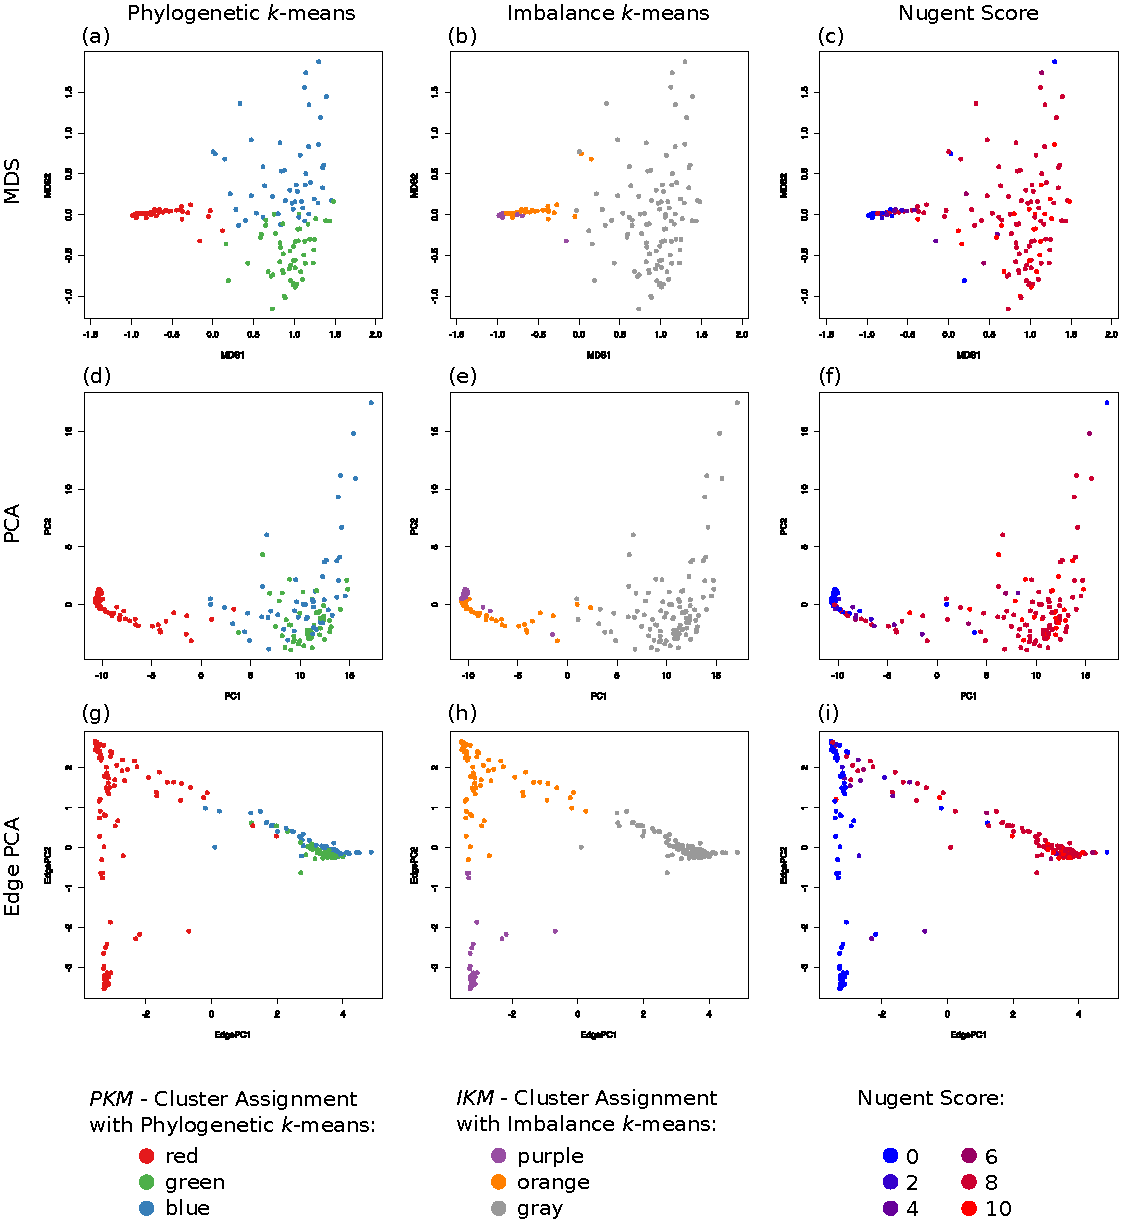
\includegraphics[width=\linewidth]{pppp/kmeans_all.pdf}
    \begin{subfigure}{0pt}
        \phantomcaption
        \label{fig:kmeans_all:sub:mds_em}
    \end{subfigure}
    \begin{subfigure}{0pt}
        \phantomcaption
        \label{fig:kmeans_all:sub:mds_ei}
    \end{subfigure}
    \begin{subfigure}{0pt}
        \phantomcaption
        \label{fig:kmeans_all:sub:mds_ns}
    \end{subfigure}
    \begin{subfigure}{0pt}
        \phantomcaption
        \label{fig:kmeans_all:sub:pca_em}
    \end{subfigure}
    \begin{subfigure}{0pt}
        \phantomcaption
        \label{fig:kmeans_all:sub:pca_ei}
    \end{subfigure}
    \begin{subfigure}{0pt}
        \phantomcaption
        \label{fig:kmeans_all:sub:pca_ns}
    \end{subfigure}
    \begin{subfigure}{0pt}
        \phantomcaption
        \label{fig:kmeans_all:sub:epca_em}
    \end{subfigure}
    \begin{subfigure}{0pt}
        \phantomcaption
        \label{fig:kmeans_all:sub:epca_ei}
    \end{subfigure}
    \begin{subfigure}{0pt}
        \phantomcaption
        \label{fig:kmeans_all:sub:epca_ns}
    \end{subfigure}
    \caption[Comparison of $k$-means clustering to MDS, PCA, and Edge PCA]{
        \textbf{Comparison of $k$-means clustering to MDS, PCA, and Edge PCA.}
        Here, we show and compare the dimensionality reduction methods MDS, PCA, and Edge PCA (one per row).
        MDS and PCA were calculated on the pairwise KR distance matrix of the \ac{BV} dataset,
        Edge PCA was calculated using the placements
        on the re-inferred \ac{RT} of the original publication \cite{Srinivasan2012}.
        The plots are colored by the cluster assignments as found by our $k$-means variants (first two columns),
        and by the Nugent score of the samples (last column).
        The Nugent score is included to allow comparison of the health status of patients with the clustering results.
        \subref{fig:kmeans_all:sub:mds_em}, \subref{fig:kmeans_all:sub:pca_em} and \subref{fig:kmeans_all:sub:epca_ei}
        are identical to \figref{fig:cluster_kmeans}\subref{fig:cluster_kmeans:sub:mds},
        \subref{fig:cluster_kmeans:sub:pca} and \subref{fig:cluster_kmeans:sub:edgepca} of the main text, respectively.
        \subref{fig:kmeans_all:sub:pca_ns} and \subref{fig:kmeans_all:sub:epca_ns} are recalculations of
        Figures~4 and 3 of \cite{Matsen2011b}, respectively.
        This figure reveals additional details about how the $k$-means method works,
        that is, which samples are assigned to the same cluster.
        For example, the purple cluster found by Imbalance $k$-means forms a dense cluster of close-by samples on the left
        in \subref{fig:kmeans_all:sub:mds_ei} and \subref{fig:kmeans_all:sub:pca_ei},
        which is in accordance with the short branch lengths
        of this cluster as shown in \figref{fig:cluster_kmeans:sub:imbalance_tree} of the main text.
    }
    \label{fig:kmeans_all}
\end{figure}

% ======================================================================================================================
%     k-means Centroids
% ======================================================================================================================

\begin{figure}[hpbt]
    \centering
    \includegraphics[width=\linewidth]{pppp/centroids.pdf}
    \caption[Example of $k$-means cluster centroids visualization]{
        % In this figure, I assume that the reader is already familiar with the characteristics of the dataset.
        % No need to repeat everything over again...
        \textbf{Example of $k$-means cluster centroids visualization.}
        Here we show the cluster centroids as found by our $k$-means variants using the \ac{BV} dataset,
        visualized on the reference tree via color coding.
        The cluster assignments are the same as in \figref{fig:cluster_kmeans} of the main text;
        the first row show the three clusters found by Phylogenetic $k$-means,
        the second row the clusters found by Imbalance $k$-means.
        Each tree represents one centroid around which the samples were clustered,
        that is, it shows the combined masses of the samples that were assigned to that cluster.
        The edges are colored relative to each other, using a linear scaling of
        light blue (no mass), purple (half of the maximal mass) and black (maximal mass).
        \\
        As explained in the main text, the samples can be split into three groups:
        The diseased subjects, which have placement mass in various parts of the tree,
        as well as two groups of healthy subjects, with placement mass in one of two \taxonname{Lactobacillus} clades
        (marked with black arcs on the left of the trees).
        This grouping is also clearly visible in these trees.
        The red cluster for example represents all healthy subjects,
        and thus most of its mass is located in the two \taxonname{Lactobacillus} clades.
        The purple and orange clusters on the other hand show a difference in placement mass between those clades.
        Furthermore, the placement mass of the gray cluster is mostly
        a combination of the masses of the green and blue cluster,
        all of which represent diseased subjects.
        These observations are in accordance with previous findings as explained in the main text.
    }
    \label{fig:centroids}
\end{figure}

% ======================================================================================================================
%     k-means HMP
% ======================================================================================================================

\begin{figure}[hpbt]
    \centering
    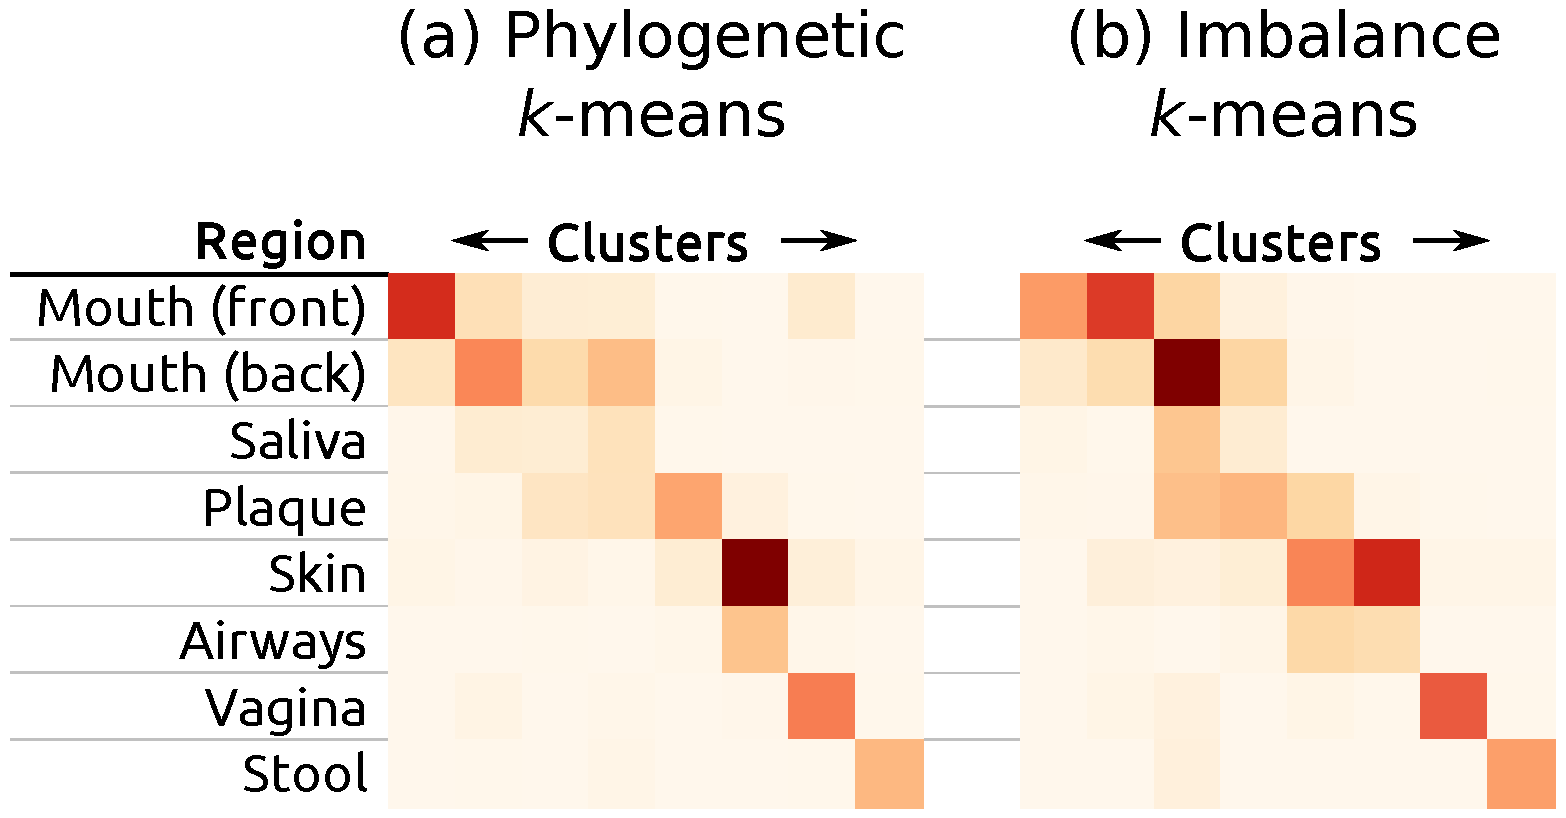
\includegraphics[width=0.6\linewidth]{pppp/hmp_kmeans_all_8.pdf}
    \caption[Clustering using Phylogenetic $k$-means on the HMP dataset]{
        \textbf{Clustering using Phylogenetic $k$-means on the HMP dataset.}
        $k$ is set to 8, instead of $k:=18$ as in the main text,
        based on a coarse aggregation of the original body site labels.
        See \figref{fig:cluster_kmeans} for the cluster assignment where $k$ is set to the original number of labels;
        there, we also list how the labels were aggregated.
        Each row represents a body site; each column one of the \num{8} clusters.
        The color values indicate how many samples of a body site were assigned to each cluster.
        Some of the body sites can be clearly separated,
        while particularly the samples from the oral region are distributed over different clusters.
        This might be due to %the broad reference tree not being able to resolve the fine details between these samples,
%         but might also indicate a
        homogeneity of the oral samples.
    }
    \label{fig:hmp_kmeans_all_8}
\end{figure}

% ======================================================================================================================
%     k-means Elbow Plots
% ======================================================================================================================

\begin{figure}[hpbt]
    \centering
    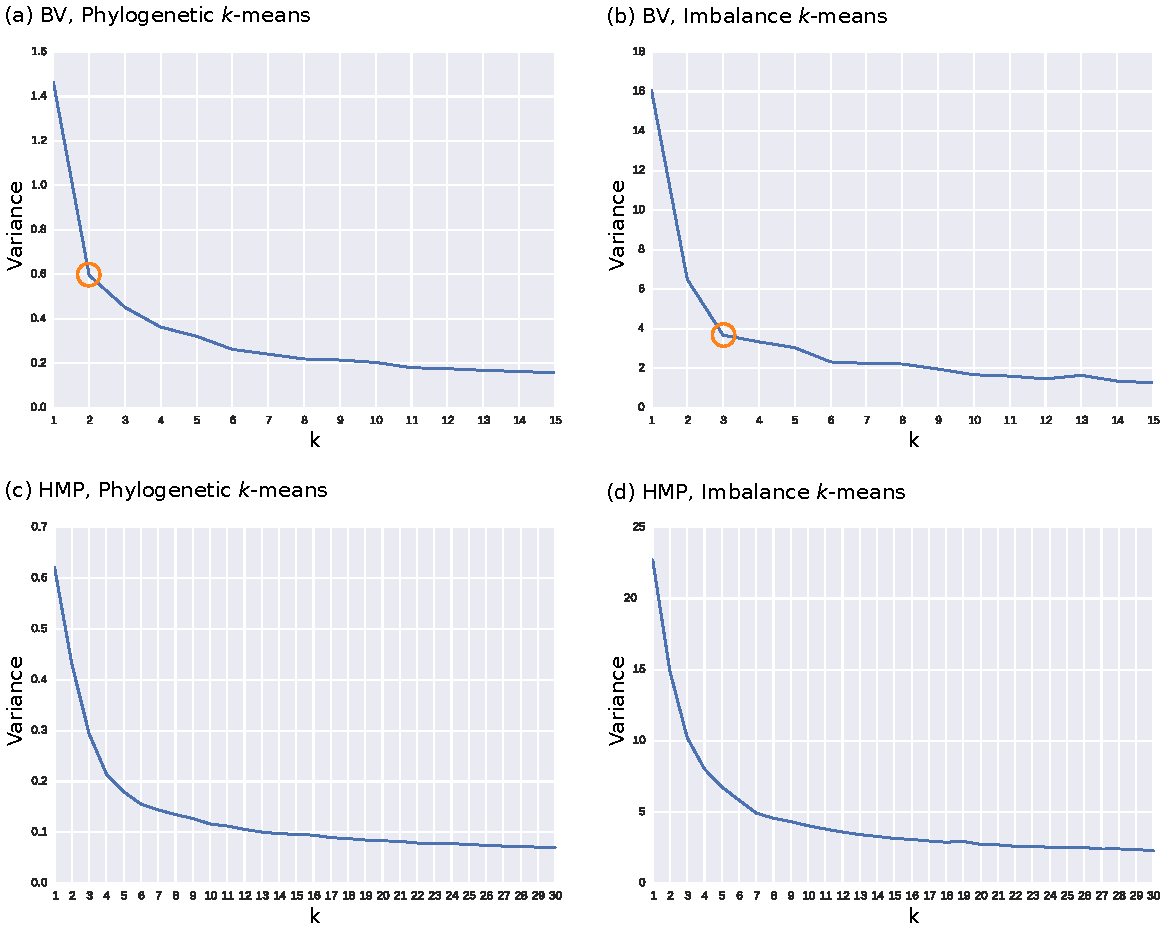
\includegraphics[width=\linewidth]{pppp/elbows.pdf}
    \begin{subfigure}{0pt}
        \phantomcaption
        \label{fig:elbows:sub:bv_phylo}
    \end{subfigure}
    \begin{subfigure}{0pt}
        \phantomcaption
        \label{fig:elbows:sub:bv_imb}
    \end{subfigure}
    \begin{subfigure}{0pt}
        \phantomcaption
        \label{fig:elbows:sub:hmp_phylo}
    \end{subfigure}
    \begin{subfigure}{0pt}
        \phantomcaption
        \label{fig:elbows:sub:hmp_imb}
    \end{subfigure}
    \caption[Variances of $k$-means clusters in our test datasets]{
        \textbf{Variances of $k$-means clusters in our test datasets.}
        The figures show the cluster variance,
        that is, the average squared distance of the samples to their assigned cluster centroids,
        for different values of $k$.
        The first row are clusterings of the BV dataset, the second row of the HMP dataset.
        They were clustered using Phylogenetic $k$-means (first column),
        and Imbalance $k$-means (second column), respectively.
        Accordingly, \subref{fig:elbows:sub:bv_phylo} and \subref{fig:elbows:sub:hmp_phylo} use the KR distance,
        while \subref{fig:elbows:sub:bv_imb} and \subref{fig:elbows:sub:hmp_imb} use the euclidean distance
        to measure the variance.
        These plots can be used for the Elbow method
        in order to find the appropriate number of clusters in a dataset \cite{Thorndike1953}.
        Low values of $k$ induce a high variance, because many samples exhibit a large distance from their assigned centroid.
        On the other hand, at a given point, higher values of $k$ only yield a marginal gain by further splitting clusters.
%         and slightly reduce this distance by further splitting clusters.
        Thus, if the data has a natural number of clusters, the corresponding $k$ produces an angle in the plot,
        called the ``elbow''.
%         Candidate points for such elbows are marked in orange here.
        \\
        For example, \subref{fig:elbows:sub:bv_phylo} and \subref{fig:elbows:sub:bv_imb}
        exhibit the elbow at $k:=2$ and $3$, respectively, which are marked with orange circles.
        These values are consistent with previous findings, for instance, \figref{fig:cluster_kmeans}:
        There, Phylogenetic $k$-means splits the samples into a distinct red cluster and the nearby green and blue clusters,
        while Imbalance $k$-means yields three separate clusters in purple, orange, and gray.
        \\
        For the HMP dataset, the elbow is less pronounced.
        We suspect that this is due to the broad reference tree not being able to adequately
        resolve fine-grained differences between samples,
        see \secref{ch:EmpiricalDatasets} for details.
        Likely candidates for $k$ are $4-6$ for \subref{fig:elbows:sub:hmp_phylo}
        and around $7$ for \subref{fig:elbows:sub:hmp_imb}.
        These values are consistent with the number of coherent ``blocks'' of clusters,
        which can be observed in \figref{fig:hmp_kmeans_all_18}.
        Clearer results for this dataset might be obtained with other methods for finding ``good'' values for $k$,
        although we did not test them here.
    }
    \label{fig:elbows}
\end{figure}
